% Expanded theoretical draft, constrained to <=13 pages including references.
\documentclass[10pt,twocolumn]{article}
\usepackage[T1]{fontenc}
\usepackage[utf8]{inputenc}
\usepackage{amsmath,amssymb,graphicx,natbib,booktabs,microtype,balance}
\usepackage[margin=1.75cm,columnsep=0.58cm]{geometry}
\usepackage[colorlinks=true,citecolor=blue,urlcolor=blue,linkcolor=blue]{hyperref}
\bibliographystyle{plainnat}
\setlength{\bibsep}{0pt}
\setlength{\parindent}{1em}
\setlength{\parskip}{0pt}
\raggedbottom
\newcommand{\Ke}{K_{\rm e}}
\newcommand{\Ki}{K_{\rm ini}}
\newcommand{\zi}{z_{\rm i}}
\newcommand{\xHI}{x_{\rm HI}}

\title{\vspace{-0.8cm}\bf Cosmic-ray electrons as ionizing agents of the
intergalactic medium during the epoch of reionization}
\author{\small Draft manuscript}
\date{}

\begin{document}
\maketitle
\vspace{-0.6cm}

\begin{abstract}
Cosmic-ray (CR) electrons accelerated by the first stellar populations cool in
an intergalactic medium (IGM) whose density, ionization state and radiation
background evolve on comparable cosmological timescales. We follow electrons
injected at $\zi=10$ and 20 down to $z=5.5$, integrating adiabatic,
synchrotron, inverse-Compton (IC), Coulomb, excitation, ionization and
bremsstrahlung losses simultaneously. The electron-impact cascade is closed
with an energy-dependent binary-encounter-dipole secondary spectrum. We then
integrate the differential Klein--Nishina spectrum of CMB photons emitted by
every cascade electron. In the approved deposition estimate, each photon from
13.6 eV to 1 keV produces one H photoionization and a photoelectron of energy
$E_\gamma-13.6$ eV, which launches the same electron cascade. Direct collisions
alone yield a minimum $W=\Ki/Y\simeq35.4$ eV near 1 keV and saturate at
$Y\simeq(0.8$--$1.2)\times10^4$. The photon branch opens at a few MeV and
creates a second efficient window near $\Ki\sim(5$--$9)\times10^7$ eV, where
$W\simeq39$ eV. It raises the high-energy plateau to $2.9\times10^6$
($\zi=20$) and $4.0\times10^6$ ($\zi=10$). Replacing 1 keV by the
redshift-dependent interaction-horizon ceiling raises these values to
$3.9\times10^6$ and $4.5\times10^6$. Thus leptonic ionization has two
productive energy windows, while its global importance remains controlled by
the injection spectrum, electron escape and photon radiative transfer.
\end{abstract}

\section{Introduction}

\subsection{Reionization and cosmic dawn}

Hydrogen reionization is the last global phase transition of the baryonic
Universe. The Ly$\alpha$ forest indicates that reionization-related
fluctuations persist to at least $z\simeq5.3$, whereas the CMB optical depth
$\tau=0.054\pm0.007$ places the midpoint of a rapid transition near
$z\simeq7.7$ and limits a substantial ionized fraction at $z\gtrsim15$
\citep{Bosman2022,Planck2020}. The range $5.5\le z\le20$ therefore brackets
the transition and the preceding cosmic-dawn interval in which the first
sources began to alter the IGM \citep{Robertson2022,Klessen2023}.

The ionizing-photon budget is still uncertain. Early galaxies are the standard
source population, but their inferred abundance, ionizing efficiency and
escape fraction can overproduce the ionization history allowed by the CMB and
Ly$\alpha$ forest, a tension often called the post-JWST photon-budget crisis
\citep{Robertson2022,Munoz2024}. Independent 21-cm limits also disfavor models
in which the neutral IGM remains at the adiabatic cooling floor until late
times, implying energy deposition before ionized regions overlap
\citep{HERA2023}. Heating and ionization by fast particles are two outcomes of
the same microscopic energy-loss problem \citep{Furlanetto2010}.

\subsection{Why cosmic-ray electrons?}

The first stellar populations provide shocks and compact remnants capable of
particle acceleration. Metal-free stars form in early minihaloes, and their
winds, supernovae and remnants inject mechanical power on timescales short
compared with the duration of reionization \citep{Klessen2023,Owen2017}.
Collisionless quasi-parallel shocks accelerate ions and electrons into
non-thermal power laws, while low metallicity enhances the output of high-mass
X-ray binaries that may also drive non-thermal outflows
\citep{Park2015,Kaur2022}. Whether these electrons reach the diffuse IGM is a
separate escape problem; throughout this paper ``injected electron'' means one
that has already escaped its host.

CR heating of the early IGM has been studied primarily for protons. Primordial
supernovae can supply sub-relativistic CRs that heat neutral gas, and
cosmological transport calculations find temperature increments of order
10--200 K by $z\sim10$ for plausible hadronic spectra, while their direct
ionization contribution remains small \citep{Sazonov2015,Leite2017}. The
spatial structure of this heating depends on diffusion and magnetic
self-confinement \citep{Jana2018,GesseyJones2023}. Electrons require a separate
calculation because IC losses on the CMB are efficient and create secondary
photons that have no hadronic analogue at fixed particle energy
\citep{Blumenthal1970,Slatyer2009}.

We calculate the ionization yield per escaped electron before convolving it
with any source spectrum. This ordering separates atomic and cosmological
physics from uncertain acceleration efficiencies. It also corrects a
limitation of the earlier draft: photon-mediated ionizations are now computed
from the differential IC spectrum rather than inferred from an energy-loss
curve.

\section{Physical model}
\label{sec:model}

\subsection{Fiducial IGM}

We adopt the approved homogeneous, pure-hydrogen baseline
\begin{equation}
 n_{\rm HI}(z)=1.8\times10^3\left(\frac{1+z}{21}\right)^3
 \mathrm{m^{-3}},\qquad x_e\equiv\frac{n_e}{n_{\rm HI}}=10^{-4},
 \label{eq:igm}
\end{equation}
and a frozen-in magnetic field
$B(z)=B_0(1+z)^2$ with $B_0=1$ nG. Cosmological ages and $H(z)$ use the
Planck-2018 cosmology as implemented in \texttt{astropy}
\citep{Planck2020,Astropy2022}. The ages at $z=20$, 10 and 5.5 are 178.1,
471.4 and 1038.5 Myr, respectively. Helium and recombinations are omitted, and
the residual ionized fraction is held fixed.

The CMB and magnetic energy densities both scale as $(1+z)^4$ under these
assumptions. In the Thomson limit their ratio is redshift-independent,
\begin{equation}
 \frac{U_B}{U_{\rm CMB}}=\frac{B_0^2}{2\mu_0U_{{\rm CMB},0}}
 =9.5\times10^{-8},                                           \label{eq:ubucmb}
\end{equation}
and equality would require $B_0\simeq3.2\,\mu$G. Klein--Nishina suppression
raises the synchrotron-to-IC ratio at the highest energies, but the numerical
loss model shows that synchrotron cooling remains dynamically negligible over
the range studied here \citep{Blumenthal1970}.

\subsection{Seven simultaneous electron losses}

For kinetic energy $\Ke$, total energy $E=\Ke+m_ec^2$ and
$p^2c^2=\Ke(\Ke+2m_ec^2)$, the trajectory is
\begin{equation}
 \frac{d\Ke}{dt}=-\sum_{j=1}^{7}L_j(z,\Ke).                    \label{eq:loss}
\end{equation}
Adiabatic redshifting gives $L_{\rm ad}=H(z)p^2c^2/E$. The
isotropic-pitch-angle synchrotron and IC rates are
\begin{equation}
 L_{\rm rad}=\frac{4}{3}\sigma_TcU\frac{p^2c^2}{(m_ec^2)^2},
 \quad U=U_B\;\hbox{or}\;U_{\rm CMB}F_{\rm KN}(b),            \label{eq:rad}
\end{equation}
where $b=4\gamma kT_{\rm CMB}/(m_ec^2)$ and $F_{\rm KN}$ is obtained by
integrating the Klein--Nishina kernel over the Planck spectrum
\citep{Blumenthal1970}. Coulomb losses on the residual plasma follow
\citet{Gould1972}. Excitation is summed over H$(1s\rightarrow np)$ for
$n=2$--10 using scaled plane-wave-Born cross-sections \citep{Stone2002}.
Collisional ionization uses the relativistic binary-encounter-Bethe (RBEB)
cross-section, with the binding energy plus the mean secondary-electron energy
removed per event \citep{Kim2000,KimRudd1994}. Bremsstrahlung uses the screened
and unscreened limits of \citet{Blumenthal1970}.

The seven rates are integrated as one stiff ordinary differential equation
with an implicit Radau method. A terminal event stops a trajectory at
$\Ke=3kT_{\rm CMB}(z)/2$. Seven augmented states simultaneously accumulate
$\int L_jdt$, ensuring that the channel fractions are evaluated on the same
trajectory and sum to the kinetic energy lost. Electrons are injected at
$\zi=10$ or 20 and followed to $z=5.5$ if they have not thermalized earlier.

\begin{figure*}[t]
\centering
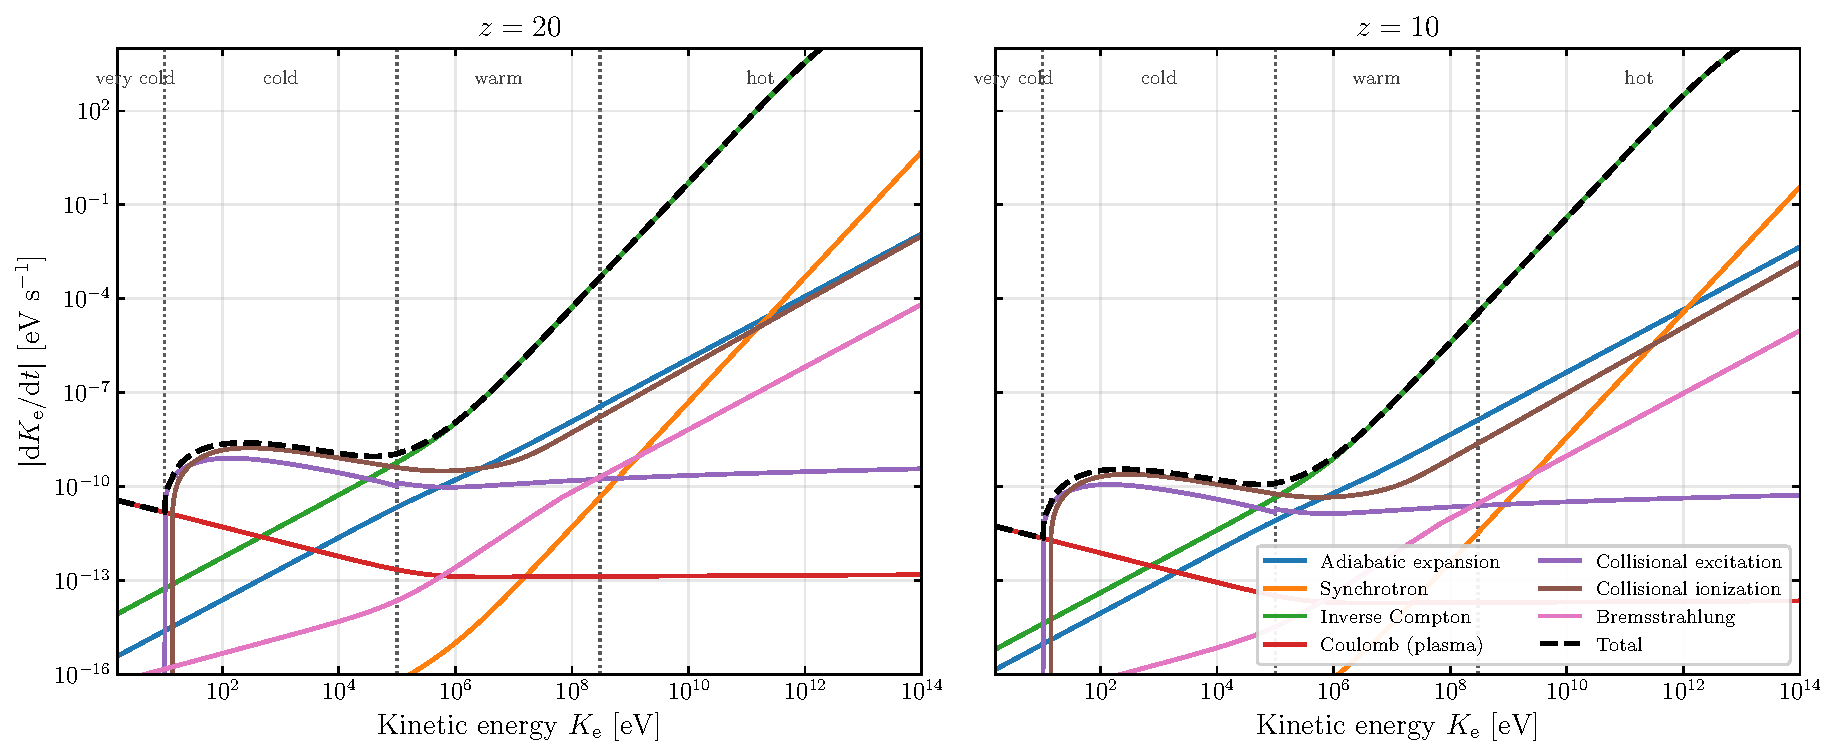
\includegraphics[width=\textwidth]{figures/fig01_loss_rates.pdf}
\caption{Instantaneous loss rates at $z=20$ and 10 for the approved IGM. The
three vertical dotted lines are the nominal conceptual divisions at 10.2 eV,
100 keV and 300 MeV; the physically computed boundaries are listed in
Table~\ref{tab:bounds}. Every curve is evaluated from the common loss module
using the cross-sections cited in Sect.~\ref{sec:model}.}
\label{fig:rates}
\end{figure*}

\section{Structure of the cooling problem}
\label{sec:structure}

\subsection{Instantaneous dominance and regime boundaries}

Figure~\ref{fig:rates} shows three broad electron-loss domains. Coulomb and
atomic losses control sub-relativistic particles, IC losses rise rapidly above
the collisional domain, and adiabatic, synchrotron and bremsstrahlung terms do
not dominate within the plotted parameter range. Instantaneous dominance does
not itself determine deposition: a cooling electron traverses several domains
before thermalization.

Four useful boundaries organize the $(z,\Ke)$ plane. $K_1=13.6057$ eV is the H
ionization threshold. $K_2$ solves
$L_{\rm ion}(z,K_2)=L_{\rm IC}(z,K_2)$ and decreases with redshift because
atomic losses scale approximately as $(1+z)^3$ whereas the CMB energy density
scales as $(1+z)^4$ \citep{Kim2000,Blumenthal1970}. $K_3$ is the electron
energy for which an up-scattered photon from the high-energy CMB percentile
first reaches 13.6 eV. $K_4$ maps the photon interaction-horizon energy,
defined by $\lambda_\gamma=c/H$, back to a parent-electron energy using the IC
kinematics \citep{Blumenthal1970,Karzas1961}.

\begin{table}[t]
\centering
\caption{Computed regime boundaries. $E_{\gamma,\rm hor}$ is the photon
energy at which the adopted interaction mean free path equals $c/H(z)$; all
other columns are electron kinetic energies in eV.}
\label{tab:bounds}
\footnotesize
\begin{tabular}{rcccc}
\toprule
$z$ & $K_2$ & $K_3$ & $E_{\gamma,\rm hor}$ & $K_4$\\
\midrule
20.0 & $7.60\!\times\!10^4$ & $4.20\!\times\!10^6$ & 1820 & $3.25\!\times\!10^8$\\
15.0 & $9.32\!\times\!10^4$ & $4.88\!\times\!10^6$ & 1550 & $3.43\!\times\!10^8$\\
10.0 & $1.23\!\times\!10^5$ & $5.99\!\times\!10^6$ & 1272 & $3.75\!\times\!10^8$\\
 8.0 & $1.43\!\times\!10^5$ & $6.67\!\times\!10^6$ & 1151 & $3.94\!\times\!10^8$\\
 5.5 & $1.82\!\times\!10^5$ & $7.93\!\times\!10^6$ &  983 & $4.29\!\times\!10^8$\\
\bottomrule
\end{tabular}
\end{table}

The photon boundary is intrinsically broad because the CMB and IC output are
spectra, not monoenergetic beams. We use $K_3$ only as a diagnostic; the photon
yield itself is always integrated over the full differential spectrum. The
fixed 1-keV absorbed band is the headline assumption approved for this work,
while $E_{\gamma,\rm hor}(z)$ is retained only as an opacity sensitivity test.

\begin{figure*}[t]
\centering
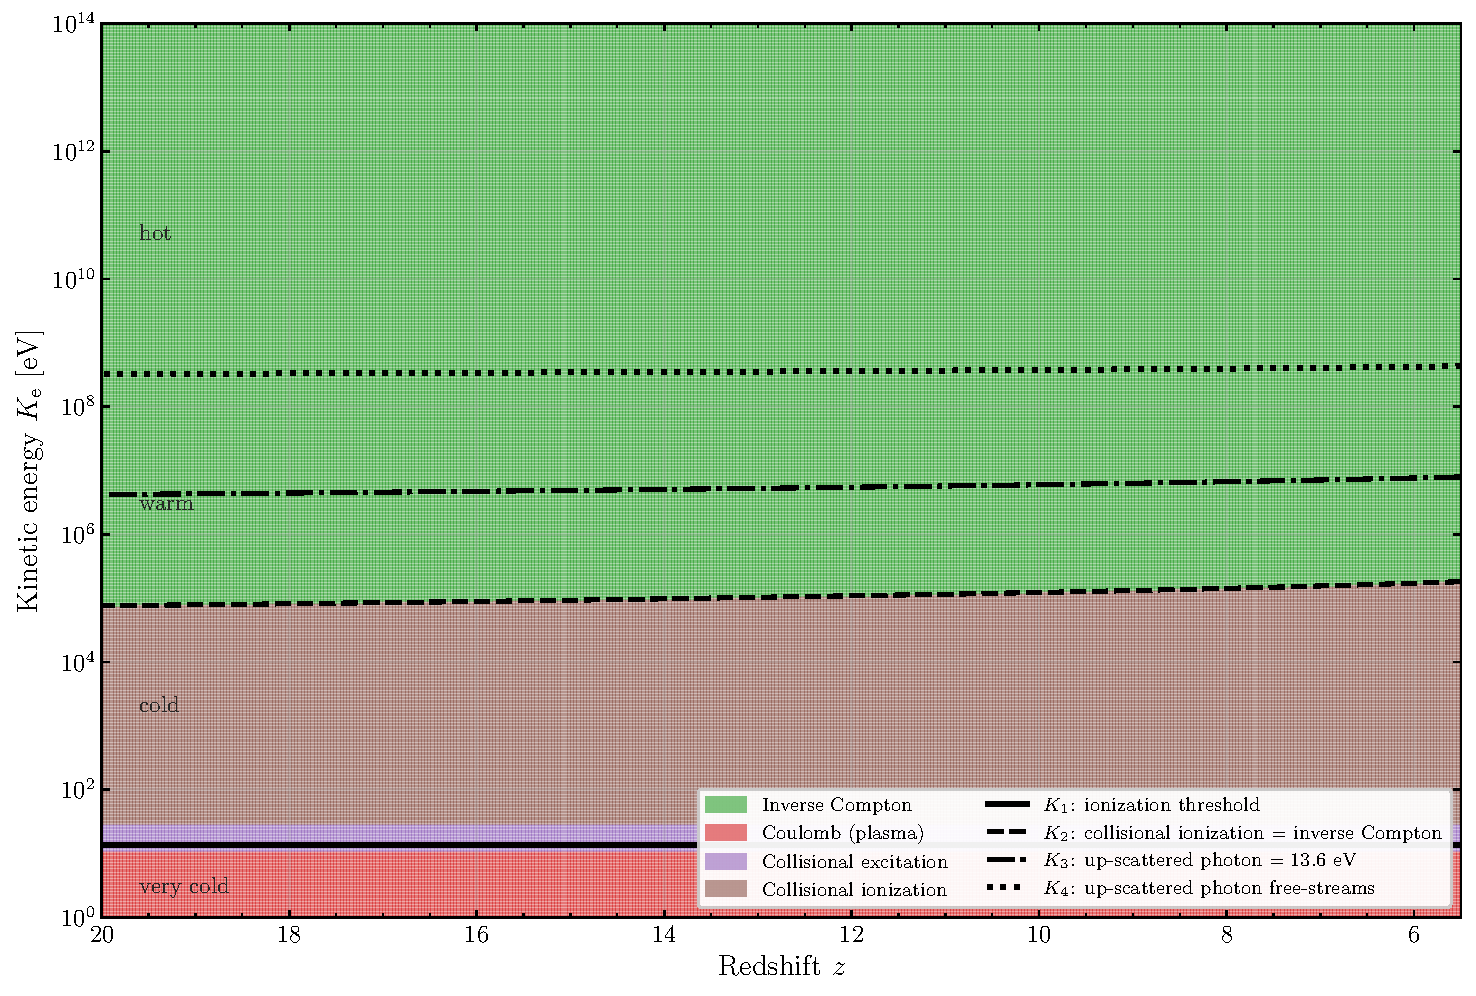
\includegraphics[width=0.82\textwidth]{figures/fig02_phase_space.pdf}
\caption{Dominant instantaneous loss channel over $5.5\le z\le20$, with the
four diagnostic boundaries. The $K_3$ and $K_4$ curves describe the fate of IC
photons rather than a change in the electron loss mechanism.}
\label{fig:phase}
\end{figure*}

\subsection{Integrated energy budgets}

The accumulated channel fractions are more informative than an instantaneous
map. At 100 eV, collisional ionization, excitation and Coulomb heating receive
approximately 0.48, 0.40 and 0.12 of the initial energy. Near 1 keV the
ionization fraction rises to about 0.68 and excitation receives 0.31. At 1 MeV
IC already receives 0.80 ($\zi=20$) or 0.66 ($\zi=10$), and above 100 MeV it
receives at least 0.99. These fractions are direct outputs of the simultaneous
integration based on \citet{Blumenthal1970,Gould1972,Stone2002,Kim2000}.

\begin{figure*}[t]
\centering
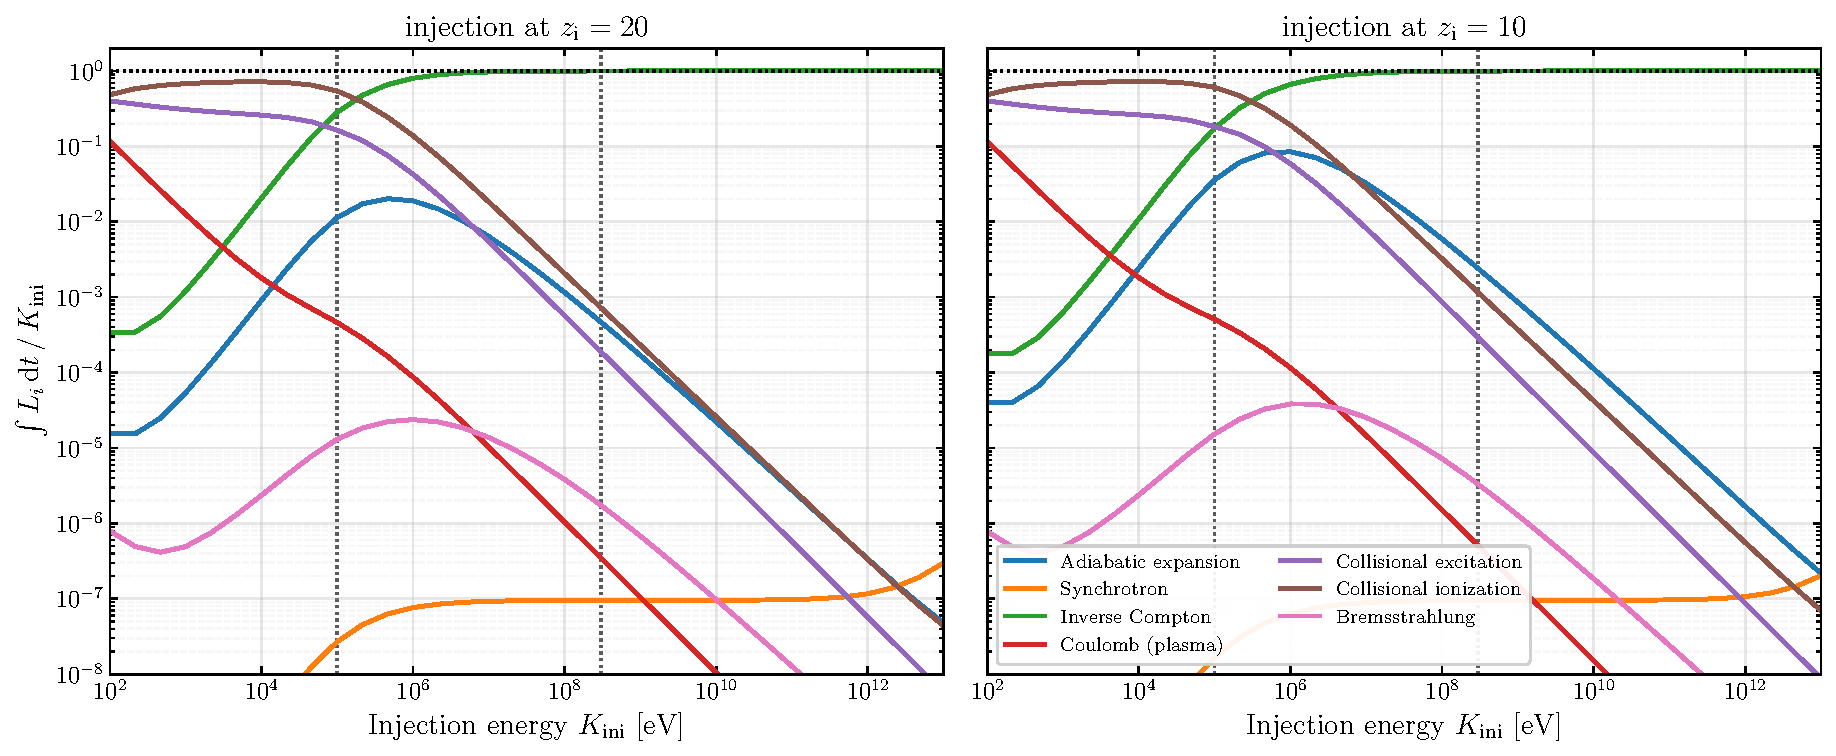
\includegraphics[width=\textwidth]{figures/fig04_energy_budget.pdf}
\caption{Fraction of the injection energy carried by each electron-loss
channel before thermalization, for $\zi=20$ and 10. IC energy in this figure is
radiated energy; only the spectral fraction inside the adopted photon band is
converted into ionizations in Sect.~\ref{sec:cascade}.}
\label{fig:budget}
\end{figure*}

The distinction in the caption is essential. Counting the entire IC loss as
locally deposited would overestimate ionization, whereas discarding it would
miss the productive 13.6 eV--1 keV photons. The differential calculation below
selects the relevant part of the radiated spectrum.

\section{Ionization cascade}
\label{sec:cascade}

\subsection{Electron-impact branch}

An ionizing electron collision creates one ion and a secondary electron. The
RBEB singly differential cross-section supplies a normalized, energy-dependent
distribution $P_{\rm sec}(\epsilon|\Ke)$ \citep{KimRudd1994}. Along a parent
trajectory the direct yield satisfies
\begin{equation}
 \dot Y_e=n_{\rm HI}v\sigma_{\rm ion}(\Ke)
 \left[1+\int d\epsilon\,P_{\rm sec}(\epsilon|\Ke)
 Y_e(\epsilon,z)\right].                                      \label{eq:electron}
\end{equation}
Because $\epsilon\le(\Ke-B_{\rm H})/2<\Ke$, the recursion is causal and can be
marched upward on an energy grid. Each generation follows Eq.~(\ref{eq:loss})
on its own cosmological trajectory. At low energy the solution agrees with
independent neutral-gas deposition calculations
\citep{Shull1985,Furlanetto2010}.

\subsection{Productive inverse-Compton photons}

For an isotropic blackbody field, the differential IC rate is
\begin{align}
 \frac{d\dot N_\gamma}{dE_\gamma}
 &=\frac{3\sigma_Tc}{4\gamma^2}
 \int d\epsilon\,\frac{n(\epsilon)}{\epsilon}G(q,\Gamma),     \label{eq:ic}\\[-2pt]
 q&=\frac{E_\gamma}{\Gamma(\gamma m_ec^2-E_\gamma)},\qquad
 \Gamma=\frac{4\gamma\epsilon}{m_ec^2},\nonumber\\[-2pt]
 G&=2q\ln q+(1+2q)(1-q)
 +\frac{(\Gamma q)^2(1-q)}{2(1+\Gamma q)},\nonumber
\end{align}
with $1/(4\gamma^2)\le q\le1$ \citep{Blumenthal1970}. Integrating
Eq.~(\ref{eq:ic}) over all output energies reproduces the IC power used in
Eq.~(\ref{eq:rad}) to 0.4 per cent at 10 MeV and to 0.2 per cent above
100 MeV. This independent energy check ensures consistency between the
trajectory and photon-counting calculations.

Following the approved hypothesis, every photon with
$B_{\rm H}=13.6057$ eV $\le E_\gamma\le E_{\max}=1$ keV produces one H
photoionization. Its photoelectron begins with
$\Ke=E_\gamma-B_{\rm H}$ and launches the same electron cascade, so
\begin{equation}
 \dot Y_\gamma=\int_{B_{\rm H}}^{E_{\max}}dE_\gamma
 \frac{d\dot N_\gamma}{dE_\gamma}
 \left[1+Y_e(E_\gamma-B_{\rm H},z)\right].                    \label{eq:photon}
\end{equation}
Equation~(\ref{eq:photon}) is evaluated for the primary and every collisional
secondary. The total is $Y=Y_e+Y_\gamma$. Photoelectrons in the adopted band
have $\Ke<1$ keV, so they do not themselves generate ionizing IC photons; their
descendants remain within the electron-impact cascade
\citep{Furlanetto2010,Slatyer2009}.

For sensitivity only, we replace 1 keV by the redshift-dependent energy where
\begin{equation}
 \lambda_\gamma^{-1}=n_{\rm HI}\sigma_{\rm pi}(E_\gamma)
 +(n_{\rm HI}+n_e)\sigma_{\rm KN}(E_\gamma)=\frac{H(z)}{c}.     \label{eq:mfp}
\end{equation}
The H photoionization and Klein--Nishina cross-sections follow
\citet{Karzas1961,Blumenthal1970}. Equation~(\ref{eq:mfp}) defines an
interaction horizon, not a complete absorption probability, because scattering
and cosmological redshifting require radiative transfer.

\section{Ionization results}
\label{sec:results}

\begin{figure*}[t]
\centering
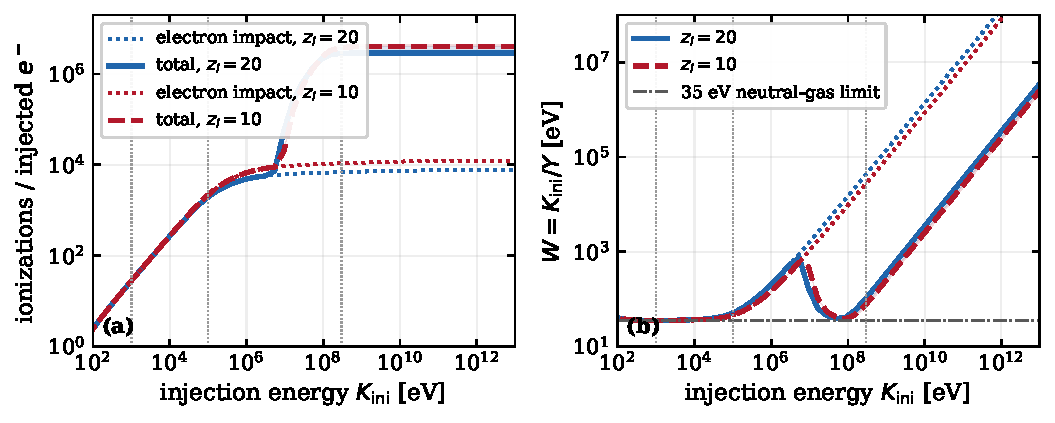
\includegraphics[width=0.98\textwidth]{figures/fig_photon_yield.pdf}
\caption{(a) Ionizations per injected electron. Dotted curves show the
electron-impact cascade; thick curves add IC photons in the 13.6 eV--1 keV band
and their photoelectron cascades. Shading extends the total to the
redshift-dependent interaction-horizon ceiling. (b) Effective energy per
ionization. The first minimum is the low-energy collisional cascade and the
second is the IC-photon window.}
\label{fig:yield}
\end{figure*}

\subsection{The direct collisional window}

Below $\sim10^5$ eV, atomic collisions control the yield. The effective energy
per ionization has a broad minimum $W\simeq35.4$ eV near 1 keV, reproducing the
neutral-gas limit of \citet{Shull1985,Furlanetto2010}. At 100 eV the cascade
produces 2.65 ionizations per electron; at 1 keV it produces 28.3. The yield is
nearly redshift-independent here because the cooling interval is much shorter
than the cosmological evolution time.

Once IC cooling overtakes collisional ionization, less primary energy reaches
the direct cascade. The electron-only result therefore flattens at
$7.7\times10^3$ ionizations for $\zi=20$ and $1.24\times10^4$ for $\zi=10$.
This plateau is the correct lower bound when emitted photons are not followed.

\subsection{The IC-photon window}

The IC spectrum develops an ionizing tail at a few MeV and dominates the
ionization count by $\Ki\sim10^7$ eV. At
$\Ki\simeq(5$--$9)\times10^7$ eV the fixed-band calculation reaches a second
minimum $W=38.7$--39.0 eV. Thus the photon branch can be almost as efficient as
the keV collisional cascade under the one-absorption prescription.

At $\Ki=2.6\times10^8$ eV the fixed photon branch produces
$2.8\times10^6$ ionizations for $\zi=20$ and $3.8\times10^6$ for $\zi=10$,
whereas direct impacts contribute only $6.9\times10^3$ and $1.1\times10^4$.
At higher $\Ki$, added energy emerges mainly above the absorbed band and the
yield saturates at $2.9\times10^6$ and $4.0\times10^6$. A productive photon
then gives 3.6 ionizations on average after its photoelectron cascade.

The interaction-horizon ceiling increases the plateaux to $3.9\times10^6$
($\zi=20$) and $4.5\times10^6$ ($\zi=10$), a 37 and 13 per cent change. This
sensitivity is modest compared with the two-to-three-order-of-magnitude
difference between the photon and direct branches, but it is large enough that
future work should replace both ceilings with radiative transfer
\citep{Slatyer2009,Slatyer2016}.

\section{Cooling histories and spatial interpretation}
\label{sec:transport}

\begin{figure*}[t]
\centering
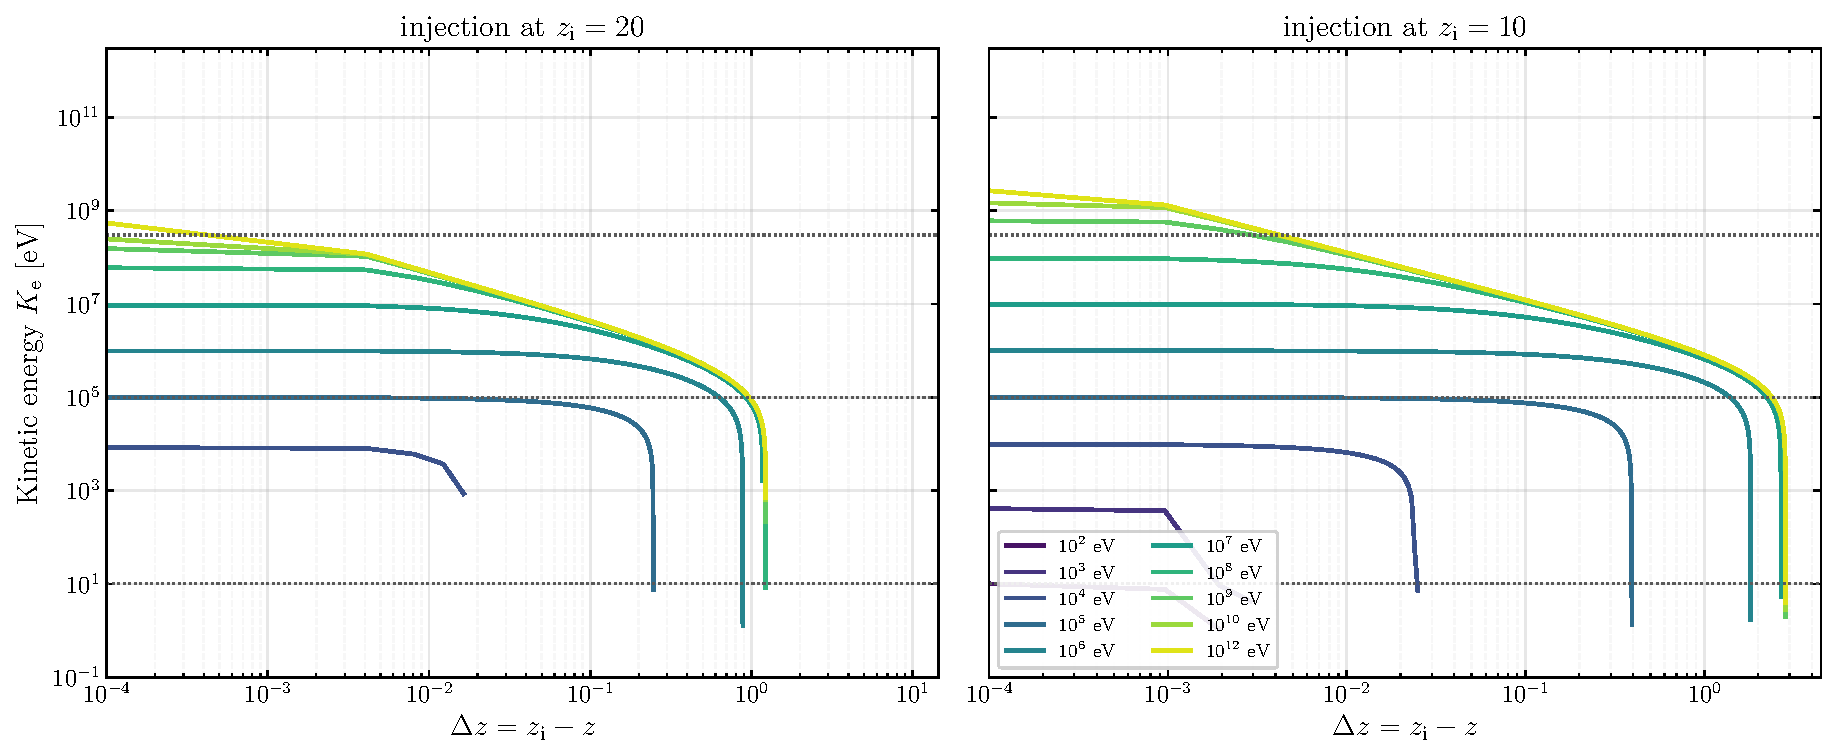
\includegraphics[width=\textwidth]{figures/fig03_cooling_histories.pdf}
\vspace{2mm}
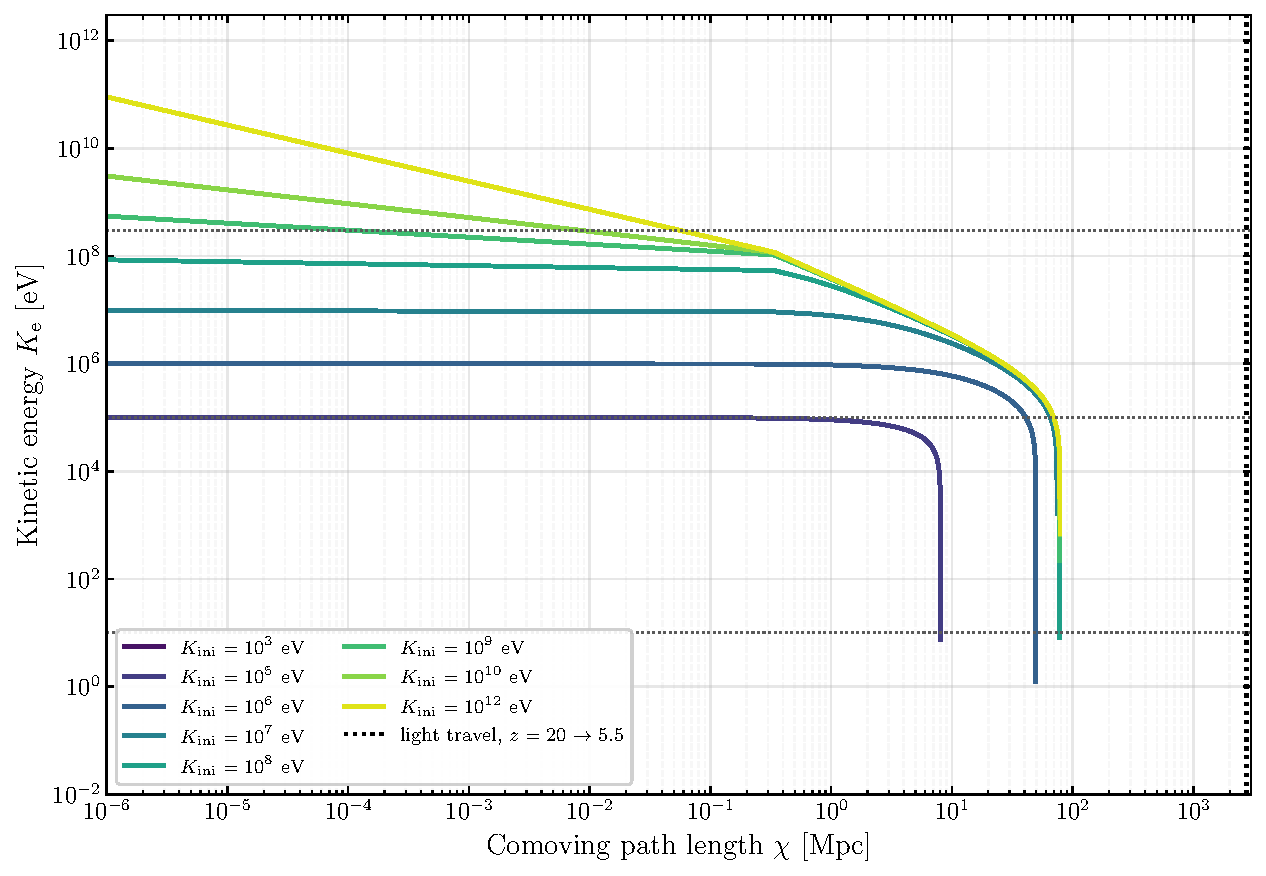
\includegraphics[width=0.62\textwidth]{figures/fig06_energy_vs_distance.pdf}
\caption{Top: electron kinetic energy against elapsed redshift interval for
injection at $\zi=20$ and 10; curves terminate at the thermal floor and
high-energy histories converge after IC cooling. Bottom: energy against
accumulated comoving path length for injection at $\zi=20$. The travel length
is not a radial displacement in a magnetized medium.}
\label{fig:cooling}
\label{fig:distance}
\end{figure*}

Cooling accelerates strongly with redshift because both gas density and the CMB
energy density increase. A 100 eV electron injected at $\zi=10$ thermalizes
after $\Delta z\simeq0.002$, whereas 1 MeV and 1 TeV electrons reach the floor
after $\Delta z\simeq1.82$ and 2.85. At $\zi=20$ the corresponding intervals
are approximately 0.001, 0.89 and 1.23. The convergence of the high-energy
histories reflects the IC-dominated descent into the same lower-energy cascade
\citep{Blumenthal1970}.

The accumulated path length is not a shell radius. For example, an electron
injected at $\zi=20$ with $10^5$ eV accumulates about 8 comoving Mpc before
thermalization, a 1 MeV electron accumulates about 50 cMpc, and injection above
$10^8$ eV approaches 78 cMpc. These are upper limits on displacement. In the
approved $B_0=1$ nG field the gyroradius is many orders of magnitude smaller,
so displacement depends on field geometry, pitch-angle scattering and the
diffusion coefficient \citep{Jana2018,Ruszkowski2023}.

Consequently, the yield calculation predicts how much ionization is produced
per electron but not where it is deposited. CR heating can be patchy for small
diffusion coefficients and more uniform for faster diffusion, a distinction
that affects 21-cm observables \citep{Jana2018,GesseyJones2023}. A spatial
source model must convolve the present yield kernel with a transport Green's
function rather than identify Fig.~\ref{fig:distance} with a bubble size.

\clearpage

\section{Injection spectra and global scaling}
\label{sec:global}

For an illustrative escaped spectrum
$dn/d\Ki=A\Ki^{-p}$ between $K_{\min}=100$ eV and
$K_{\max}=1$ TeV, the spectrum-averaged energy per ionization is
\begin{equation}
 \overline W(p)=\frac{\int_{K_{\min}}^{K_{\max}}\Ki^{1-p}d\Ki}
 {\int_{K_{\min}}^{K_{\max}}\Ki^{-p}Y(\Ki)d\Ki}.              \label{eq:wbar}
\end{equation}
The normalization $A$ cancels exactly. Power-law injection is motivated by
diffusive shock acceleration, but the extrapolation to 100 eV is illustrative
and should not be mistaken for a universal source spectrum \citep{Park2015}.

\begin{table}[t]
\centering
\caption{Spectrum-averaged energy per ionization $\overline W$ [eV] for
$100\,\mathrm{eV}\le\Ki\le1\,\mathrm{TeV}$. ``Direct'' omits IC-photon
ionizations, ``1 keV'' uses the approved fixed band, and ``horizon'' uses the
redshift-dependent ceiling of Eq.~(\ref{eq:mfp}).}
\label{tab:wbar}
\resizebox{\columnwidth}{!}{%
\begin{tabular}{r rrr rrr}
\toprule
&\multicolumn{3}{c}{$\zi=20$}&\multicolumn{3}{c}{$\zi=10$}\\
\cmidrule(lr){2-4}\cmidrule(lr){5-7}
$p$ & Direct & 1 keV & Horizon & Direct & 1 keV & Horizon\\
\midrule
1.8 & 888 & 290 & 263 & 804 & 271 & 260\\
2.0 & 107 & 79.8 & 77.4 & 102 & 77.1 & 76.2\\
2.2 & 46.3 & 44.2 & 44.0 & 45.3 & 43.5 & 43.4\\
2.5 & 37.8 & 37.7 & 37.7 & 37.6 & 37.5 & 37.5\\
3.0 & 37.4 & 37.4 & 37.4 & 37.4 & 37.4 & 37.4\\
\bottomrule
\end{tabular}}
\end{table}

Table~\ref{tab:wbar} shows that photon-mediated ionization matters most for
hard spectra that place appreciable particle number in the tens-of-MeV window.
For $p=1.8$, the fixed band lowers $\overline W$ by a factor of about three;
for $p\ge2.5$, low-energy electrons dominate both integrals and the result is
unchanged. Even after adding the productive band, energy injected far above
the plateau raises the numerator without proportionally increasing the yield.

If a source model supplies a comoving escaped-electron energy density
$u_{e,\rm CR}$ with a specified spectrum, the no-recombination ionization
density is $n_{\rm ion}=u_{e,\rm CR}/\overline W$. Turning this into a global
ionized fraction requires an evolving source history, recombinations, H/He
chemistry and spatial overlap. Existing hadronic heating normalizations cannot
be transferred directly to the electron component because the acceleration
efficiency and escape fraction differ \citep{Leite2017,Ruszkowski2023}.

\section{Discussion and limitations}

The calculation establishes two productive leptonic windows. Near keV
energies, direct H collisions generate the familiar neutral-gas cascade. Near
tens of MeV, IC photons inside the adopted absorption band produce a second
cascade with comparable $W$. Between these windows the IC spectrum is only
partly ionizing, and above the second window additional radiated energy moves
beyond the assumed absorption ceiling \citep{Blumenthal1970,Slatyer2009}.

The magnitude of the new branch is conditional on the approved photon rule.
One absorption per 13.6 eV--1 keV photon is a transparent limiting estimate,
not a self-consistent opacity solution. A full treatment must redshift photons,
distinguish absorption from Compton scattering, evolve the neutral fraction,
include helium, and follow delayed deposition across the changing IGM
\citep{Kanzaki2008,Slatyer2016}. The 13--37 per cent change produced by the
interaction-horizon ceiling quantifies only one part of that uncertainty.

The homogeneous fixed-$x_e$ approximation is likewise restrictive. Increasing
$x_e$ strengthens Coulomb heating and weakens the ionization share of
low-energy secondaries; helium adds excitation, ionization and opacity channels
\citep{Furlanetto2010}. Recombinations make one ionization per H atom
insufficient for sustained reionization, while source clustering and diffusion
control whether deposition is local or volume-filling
\citep{Robertson2022,Jana2018}.

Finally, the calculation begins after electron escape. The global impact may
be small even when the per-particle yield is high if host columns stop
sub-relativistic electrons or if accelerators place little power in either
productive window. Conversely, a soft escaped spectrum or a component near
tens of MeV can exploit the minima in Fig.~\ref{fig:yield}. Source-specific
escape and acceleration models are therefore the next necessary layer
\citep{Park2015,Ruszkowski2023}.

\section{Conclusions}

We have combined cosmological CR-electron cooling, a recursive
electron-impact cascade and the differential IC photon spectrum. The main
results are:
\begin{enumerate}
\item The direct cascade has a minimum $W\simeq35.4$ eV near 1 keV and
saturates at $(0.8$--$1.2)\times10^4$ ionizations per injected electron,
consistent with neutral-gas deposition calculations
\citep{Shull1985,Furlanetto2010}.
\item Under one absorption per 13.6 eV--1 keV photon, IC emission creates a
second minimum $W\simeq39$ eV near $(5$--$9)\times10^7$ eV and raises the
plateau to $2.9\times10^6$ ($\zi=20$) or $4.0\times10^6$ ($\zi=10$).
\item A redshift-dependent interaction-horizon ceiling increases those
plateaux to $3.9\times10^6$ and $4.5\times10^6$, demonstrating a 13--37 per
cent opacity sensitivity but not replacing radiative transfer
\citep{Karzas1961,Slatyer2016}.
\item The photon branch reduces $\overline W$ most strongly for hard injection
spectra; soft spectra remain controlled by the keV collisional window.
\item Path length is only an upper limit on displacement. A global prediction
requires source escape, magnetic transport, recombinations and photon transfer
\citep{Jana2018,Ruszkowski2023}.
\end{enumerate}

\section*{Code, algebra and reproducibility}
The common loss model, direct cascade, photon cascade and figures are in
\texttt{igm\_losses.py}, \texttt{cascade\_traj.py},
\texttt{photon\_cascade.py}, \texttt{make\_paper\_figures.py} and
\texttt{make\_short\_paper\_figure.py}. Symbolic checks are in
\texttt{verify\_manuscript\_algebra.py}; numerical text--table--figure
regressions are in \texttt{verify\_manuscript\_consistency.py}.

\footnotesize
\balance
\bibliography{references}
\end{document}
